\chapter{One-Dimensional Bar and Rod Elements}
\label{ch:1d}

\section{Direct Formulation of the Bar Element}
\label{sec:direct_formulation}

The simplest finite element is the two-node bar (rod) element, suitable for
axially loaded members. Consider an element of length $L$, cross-sectional
area $A$, and Young's modulus $E$, with nodes 1 and 2 having axial
displacements $u_1$ and $u_2$~\cite{logan2011first,cook2002concepts}.

Rather than starting from a variational principle, we derive the element
stiffness directly from \emph{mechanics of materials}: equilibrium of axial
forces combined with Hooke's law. The principle of virtual work, derived
later in this chapter (\cref{sec:pvw}), reproduces the same stiffness matrix
and provides the variational foundation for the entire finite element method.

\begin{figure}[htbp]
\centering
\begin{tikzpicture}[>=Stealth, x=1cm, y=1cm,
    disp/.style={->,very thick,blue!70!black},
    force/.style={->,ultra thick,red!75!black}]
  %% Bar body
  \fill[gray!22] (0,-0.28) rectangle (6.5,0.28);
  \draw[thick] (0,-0.28) rectangle (6.5,0.28);
  %% Material label (above bar)
  \node[above=3pt] at (3.25,0.28) {$E,\ A$};
  %% Nodes
  \filldraw (0,0) circle (4pt);
  \filldraw (6.5,0) circle (4pt);
  %% Node numbering (outside bar, below corners)
  \node at (-0.30,-0.50) {\small\bfseries 1};
  \node at (6.80,-0.50) {\small\bfseries 2};
  %% Displacement arrows (blue, above bar) at each node
  \draw[disp] (0,0.70) -- ++(1.30,0) node[above,midway] {$u_1$};
  \draw[disp] (6.5,0.70) -- ++(1.30,0) node[above,midway] {$u_2$};
  %% Force arrows (red, below bar) at each node
  \draw[force] (0,-1.05) -- ++(1.30,0) node[below,midway] {$F_1$};
  \draw[force] (6.5,-1.05) -- ++(1.30,0) node[below,midway] {$F_2$};
  %% Length dimension
  \draw[<->,thin] (0,-1.70) -- (6.5,-1.70);
  \node[fill=white,inner sep=1pt] at (3.25,-1.70) {$L$};
  %% x-axis
  \draw[->,thin] (-0.70,-2.20) -- (8.20,-2.20) node[right] {$x$};
\end{tikzpicture}
\caption{Two-node bar element: nodal displacements $u_1$, $u_2$ (blue, above) and external nodal forces $F_1$, $F_2$ (red, below), with cross-section $A$, modulus $E$, length $L$.}
\label{fig:bar_element}
\end{figure}

\subsection{Element Kinematics}

For small deformations, the axial elongation of the element is the difference
of nodal displacements:
\begin{equation}
    \Delta L = u_2 - u_1 .
    \label{eq:bar_elongation}
\end{equation}
Assuming the strain is uniform along the element (consistent with linear
displacement variation between nodes),
\begin{equation}
    \varepsilon = \frac{\Delta L}{L} = \frac{u_2 - u_1}{L} .
    \label{eq:bar_strain_direct}
\end{equation}
Hooke's law and the axial force resultant $N = \sigma A$ give
\begin{equation}
    \sigma = E\varepsilon = \frac{E(u_2-u_1)}{L},
    \qquad
    N = \frac{EA(u_2-u_1)}{L} .
    \label{eq:bar_axial_force_direct}
\end{equation}

\subsection{Stiffness Matrix from Equilibrium}

Taking $N>0$ in tension, the external nodal forces required to produce the
displacements $u_1, u_2$ are
\begin{align}
    F_1 &= -N = \frac{EA}{L}(u_1 - u_2),
    \label{eq:bar_F1_direct} \\
    F_2 &= +N = \frac{EA}{L}(u_2 - u_1) .
    \label{eq:bar_F2_direct}
\end{align}
Collecting these in matrix form,
\begin{equation}
    \begin{bmatrix} F_1 \\ F_2 \end{bmatrix}
    = \frac{EA}{L}
    \begin{bmatrix} 1 & -1 \\ -1 & 1 \end{bmatrix}
    \begin{bmatrix} u_1 \\ u_2 \end{bmatrix}
    \quad\Longleftrightarrow\quad
    \matr{k}^e\,\vect{u}^e = \vect{f}^e .
\end{equation}
The element stiffness matrix is therefore
\begin{equation}
    \matr{k}^e = \frac{EA}{L}\begin{bmatrix} 1 & -1 \\ -1 & 1 \end{bmatrix} .
    \label{eq:bar_stiffness}
\end{equation}

\begin{importantbox}
\begin{equation*}
    \matr{k}^e = \frac{EA}{L}\begin{bmatrix} 1 & -1 \\ -1 & 1 \end{bmatrix}
\end{equation*}
\end{importantbox}

\subsection{Unit Displacement Interpretation}

The columns of $\matr{k}^e$ have a clear physical meaning. Set $u_1=1$ and
$u_2=0$: the bar shortens, the strain is $\varepsilon = -1/L$, and the internal
force is $N = -EA/L$ (compression). Equilibrium then requires the external
forces $F_1 = +EA/L$ at node 1 and $F_2 = -EA/L$ at node 2 — exactly the first
column of $\matr{k}^e$. The second column follows from $u_1=0,\ u_2=1$ by an
identical argument.

\begin{remark}
The stiffness matrix is symmetric (Maxwell's reciprocal theorem) and singular
because rows sum to zero: a uniform translation $u_1=u_2=c$ produces no
strain and no force, reflecting the rigid-body mode of the unconstrained
element.
\end{remark}

\section{Displacement Field Approximation}
\label{sec:displacement_field}

The direct formulation has used only nodal displacements. To analyze the
response \emph{between} nodes — for postprocessing strains and stresses, or for
representing distributed loading — we need an approximate displacement field
$u(x)$.

\subsection{Linear Shape Functions}

The displacement field consistent with the constant-strain assumption used in
\cref{eq:bar_strain_direct} is linear in $x$:
\begin{equation}
    u(x) = N_1(x)\,u_1 + N_2(x)\,u_2 = \vect{N}\,\vect{u}^e
    \label{eq:bar_disp}
\end{equation}
with the linear Lagrange shape functions
\begin{equation}
    N_1(x) = 1 - \frac{x}{L}, \qquad N_2(x) = \frac{x}{L},
    \qquad x \in [0,L] .
    \label{eq:bar_shape}
\end{equation}

\begin{remark}
Shape functions satisfy the \emph{partition of unity}, $N_1 + N_2 = 1$, and the
\emph{Kronecker delta property}, $N_i(x_j) = \delta_{ij}$.
\end{remark}

The strain operator follows by differentiation,
\begin{equation}
    \varepsilon(x) = \frac{\dd u}{\dd x} = \matr{B}\,\vect{u}^e,
    \qquad
    \matr{B} = \frac{1}{L}\begin{bmatrix} -1 & 1 \end{bmatrix} ,
    \label{eq:bar_strain}
\end{equation}
which recovers $\varepsilon = (u_2-u_1)/L$, in agreement with
\cref{eq:bar_strain_direct}.

\subsection{Enrichment by a Particular Solution}

The strong form of the loaded bar, derived in \cref{ch:weighted_residuals}, is
\begin{equation}
    -EA\,\frac{\dd^2 u}{\dd x^2} = p(x), \qquad 0 < x < L .
    \label{eq:bar_de}
\end{equation}
The linear interpolation \cref{eq:bar_disp} solves the \emph{homogeneous}
equation $u'' = 0$ exactly, but cannot represent the inhomogeneous response
when $p(x) \neq 0$.

To recover the exact response within the element, augment the linear field
with a \emph{particular solution} $u_p(x)$:
\begin{equation}
    u(x) = N_1(x)\,u_1 + N_2(x)\,u_2 + u_p(x) ,
    \label{eq:bar_disp_enriched}
\end{equation}
where $u_p(x)$ satisfies the inhomogeneous equation with homogeneous endpoint
conditions:
\begin{equation}
    -EA\,u_p''(x) = p(x), \qquad u_p(0) = 0, \qquad u_p(L) = 0 .
    \label{eq:up_bvp}
\end{equation}
The boundary conditions on $u_p$ ensure that the linear part still recovers the
nodal displacements at the endpoints, $u(0)=u_1$ and $u(L)=u_2$.

\begin{importantbox}
\textbf{Enriched trial function:}
\begin{equation*}
    u(x) = N_1(x)\,u_1 + N_2(x)\,u_2 + u_p(x) .
\end{equation*}
The first two terms carry the nodal displacements. The particular solution
$u_p(x)$ carries the local response to the distributed load — solved once
analytically per load case and added to every element under that loading.
\end{importantbox}

\subsection{Worked Example: Uniform Distributed Load}
\label{sec:bar_uniform_load}

For a uniform distributed axial load $p(x) = p_0$, integrating
\cref{eq:up_bvp} twice and applying $u_p(0)=u_p(L)=0$ gives
\begin{equation}
    u_p(x) = \frac{p_0\,x(L - x)}{2EA} .
    \label{eq:up_uniform}
\end{equation}
This is a parabolic profile peaking at midspan with
$u_p(L/2) = p_0 L^2/(8EA)$. Substituting into \cref{eq:bar_disp_enriched}
gives the complete element displacement field for a uniformly loaded bar:
\begin{equation}
    u(x) = \left(1-\frac{x}{L}\right)u_1
         + \frac{x}{L}\,u_2
         + \frac{p_0\,x(L-x)}{2EA} .
    \label{eq:bar_disp_uniform}
\end{equation}
Differentiating once gives the axial strain
\begin{equation}
    \varepsilon(x) = \frac{u_2-u_1}{L}
                  + \frac{p_0(L-2x)}{2EA} ,
    \label{eq:bar_strain_enriched}
\end{equation}
and the internal axial force
\begin{equation}
    N(x) = EA\,\varepsilon(x)
         = \frac{EA(u_2-u_1)}{L} + \frac{p_0(L-2x)}{2} .
    \label{eq:bar_force_enriched}
\end{equation}

\section{Element Load Vector}

External forces at the element ends follow from equilibrium with the internal
axial force in \cref{eq:bar_force_enriched}: $F_1 = -N(0)$ and $F_2 = +N(L)$.
Substituting,
\begin{align}
    F_1 &= \frac{EA}{L}(u_1-u_2) - \frac{p_0 L}{2}, \\
    F_2 &= \frac{EA}{L}(u_2-u_1) - \frac{p_0 L}{2} .
\end{align}
Rearranging into the standard finite element form,
\begin{equation}
    \matr{k}^e\,\vect{u}^e = \vect{f}^e ,
    \qquad
    \vect{f}^e = \frac{p_0 L}{2}\begin{bmatrix} 1 \\ 1 \end{bmatrix} .
    \label{eq:bar_load}
\end{equation}
Half of the total distributed load is placed at each node, recovering the
familiar consistent load vector. Note that the same vector is obtained from
the variational expression $\vect{f}^e = \int_0^L \vect{N}\transpose p\,\dd x$
used in \cref{ch:weighted_residuals} and in the PVW derivation of
\cref{sec:pvw} — direct mechanics, weak form, and PVW all agree.

\begin{remark}
For constant $EA$ and uniform $p_0$, the enriched element with $u_p(x)$ is
\emph{nodally exact}: even a single element gives the exact analytical
displacement and stress at the nodes. Refining the mesh only improves the
resolution of the smooth interior fields, not the nodal accuracy.
\end{remark}

\section{Global Assembly}

Consider a bar discretized into $n$ elements with $n+1$ nodes. Each element
connects local nodes 1--2 to global nodes $i$-$(i+1)$. The global stiffness
matrix $\stiff \in \mathbb{R}^{(n+1)\times(n+1)}$ is assembled by the
\emph{direct stiffness method}:
\begin{equation}
    \stiff = \sum_{e=1}^{n} \matr{L}_e\transpose \matr{k}^e \matr{L}_e
    \label{eq:assembly}
\end{equation}
where $\matr{L}_e$ is the Boolean connectivity matrix that maps local to global DOFs.

In practice, assembly is performed by adding element stiffness entries at the
appropriate global positions:
\begin{equation}
    K_{ij} \mathrel{+}= k^e_{rs}, \quad \text{where } i = \text{global}(r),\; j = \text{global}(s)
\end{equation}

\section{Boundary Conditions}

\subsection{Homogeneous Essential BC (fixed node)}
Zero out the row and column corresponding to the prescribed DOF, and set the
diagonal to 1:
\begin{equation}
    K_{ii} = 1, \quad K_{ij} = K_{ji} = 0 \;\forall j \neq i, \quad f_i = 0
\end{equation}

\subsection{Penalty Method}
Add a large number $\alpha \gg \max(K_{ii})$ to the diagonal:
\begin{equation}
    K_{ii} \mathrel{+}= \alpha, \quad f_i \mathrel{+}= \alpha \bar{u}_i
\end{equation}
where $\bar{u}_i$ is the prescribed displacement.

\section{Worked Example: Three-Element Bar}

\begin{example}[Three-element bar under tip load]
\label{ex:3bar}

Consider a stepped bar of total length $L = 0.9$ m fixed at $x=0$,
with a point load $F = 10{,}000$ N at $x = L$. Three equal elements,
$EA = 70 \times 10^6$ N.

\medskip
\noindent\textbf{Element stiffness:}
\[
    \matr{k}^e = \frac{EA}{L/3} = \frac{70\times10^6}{0.3}
    \begin{bmatrix}1&-1\\-1&1\end{bmatrix}
    = 2.\overline{3}\times10^8
    \begin{bmatrix}1&-1\\-1&1\end{bmatrix}
\]

\noindent\textbf{Global system} (4 DOFs, node 1 fixed):
\[
    \stiff = 2.\overline{3}\times10^8
    \begin{bmatrix}
         1 & -1 &  0 &  0 \\
        -1 &  2 & -1 &  0 \\
         0 & -1 &  2 & -1 \\
         0 &  0 & -1 &  1
    \end{bmatrix},
    \qquad \vect{f} = \begin{bmatrix}0\\0\\0\\10000\end{bmatrix}
\]

\noindent\textbf{Applying BC} $u_1 = 0$ (strike row/column 1):
\[
    \vect{u} = \stiff\inv \vect{f}
    \implies u_4 = \frac{FL}{EA} = 1.286 \times 10^{-4}\ \text{m}
\]

\begin{figure}[htbp]
\centering
\begin{tikzpicture}[>=Stealth, scale=1.0]
  %% Fixed wall
  \fill[pattern=north east lines] (-0.35,-0.35) rectangle (0,0.35);
  \draw[thick] (0,-0.35) -- (0,0.35);
  %% Three bar segments (each width 2.8)
  \fill[gray!20] (0,-0.18) rectangle (2.8,0.18);
  \draw[thick] (0,-0.18) rectangle (2.8,0.18);
  \fill[gray!20] (2.8,-0.18) rectangle (5.6,0.18);
  \draw[thick] (2.8,-0.18) rectangle (5.6,0.18);
  \fill[gray!20] (5.6,-0.18) rectangle (8.4,0.18);
  \draw[thick] (5.6,-0.18) rectangle (8.4,0.18);
  %% Element labels
  \node[above=3pt] at (1.4,0.18) {\small $e=1$};
  \node[above=3pt] at (4.2,0.18) {\small $e=2$};
  \node[above=3pt] at (7.0,0.18) {\small $e=3$};
  %% Nodes
  \foreach \x/\n in {0/1,2.8/2,5.6/3,8.4/4}{
    \filldraw (\x,0) circle (3.5pt);
    \node[below=5pt] at (\x,0) {\small $\n$};
  }
  %% Le dimensions
  \foreach \s in {0,2.8,5.6}{
    \draw[<->] (\s,-0.65) -- (\s+2.8,-0.65) node[midway,below] {\small $L_e$};
  }
  %% Tip force
  \draw[->,very thick,red!70!black] (9.8,0) -- (8.4,0);
  \node[right] at (9.8,0) {$F$};
\end{tikzpicture}
\caption{Three-element bar discretization: fixed at node 1, tip load $F$ at node 4.}
\label{fig:3bar}
\end{figure}

\noindent See \Cref{lst:bar1d} in the Appendix for the MATLAB implementation.
\end{example}

\section{Worked Example: Stepped Bar with Combined Loading}
\label{sec:stepped_bar}

\begin{example}[Stepped axial bar with distributed and concentrated loads]
\label{ex:stepped_bar}

A cantilever stepped bar comprises two prismatic segments. Element~1 has
length $L_1 = 500$~mm and area $A = 225$~mm$^2$; element~2 has length
$L_2 = 400$~mm and area $2A = 450$~mm$^2$. The Young's modulus is
$E = 210{,}000$~MPa. A uniform distributed axial load $p_1 = -4$~N/mm acts on
element~1 (negative = directed toward the fixed support), and concentrated
forces of $+6$~kN at node~2 and $-15$~kN at node~3 are applied
(\cref{fig:stepped_bar}).

\begin{figure}[htbp]
\centering
\begin{tikzpicture}[>=Stealth, x=1cm, y=1cm,
    distload/.style={->,thick,blue!75!black},
    concforce/.style={->,ultra thick,red!75!black},
    dim/.style={<->,thin}]
  %% Fixed wall (hatched)
  \fill[pattern=north east lines, pattern color=gray!70] (-0.40,-0.65) rectangle (0,0.65);
  \draw[thick] (0,-0.65) -- (0,0.65);
  %% Element 1 (thinner) from x=0 to x=5 (represents 500 mm)
  \fill[gray!22] (0,-0.18) rectangle (5,0.18);
  \draw[thick] (0,-0.18) rectangle (5,0.18);
  \node[below=2pt] at (2.5,-0.18) {\small $A$};
  %% Element 2 (thicker) from x=5 to x=9 (represents 400 mm)
  \fill[gray!22] (5,-0.32) rectangle (9,0.32);
  \draw[thick] (5,-0.32) rectangle (9,0.32);
  \node[below=2pt] at (7,-0.32) {\small $2A$};
  %% Distributed load arrows over element 1 (point LEFT)
  \foreach \x in {0.6,1.3,2.0,2.7,3.4,4.1,4.8}
    \draw[distload] (\x,0.65) -- ++(-0.55,0);
  \node[blue!75!black,above] at (2.5,0.80) {$4$~kN/m};
  %% Concentrated 6 kN at node 2 (points RIGHT)
  \draw[concforce] (4.55,0.55) -- (5.55,0.55);
  \node[red!75!black,above] at (5.05,0.65) {$6$~kN};
  %% Concentrated 15 kN at node 3 (points LEFT — applied at the free end)
  \draw[concforce] (10.10,0) -- (9.10,0);
  \node[red!75!black,above] at (9.60,0.05) {$15$~kN};
  %% Nodes
  \filldraw (0,0) circle (3pt);
  \filldraw (5,0) circle (3pt);
  \filldraw (9,0) circle (3pt);
  %% Node numbering
  \node at (-0.30,-0.92) {\small\bfseries 1};
  \node at (5.00,-0.92) {\small\bfseries 2};
  \node at (9.30,-0.92) {\small\bfseries 3};
  %% Length dimensions
  \draw[dim] (0,-1.45) -- (5,-1.45);
  \node[fill=white,inner sep=1pt] at (2.5,-1.45) {\small $500$~mm};
  \draw[dim] (5,-1.45) -- (9,-1.45);
  \node[fill=white,inner sep=1pt] at (7,-1.45) {\small $400$~mm};
  %% x-axis
  \draw[->,thin] (-0.6,-2.00) -- (10.7,-2.00) node[right] {$x$};
\end{tikzpicture}
\caption{Stepped bar problem: distributed axial load (blue) on element 1 and concentrated forces (red) at nodes 2 and 3.}
\label{fig:stepped_bar}
\end{figure}

\paragraph{Discretization.}
Two linear bar elements connect three nodes located at $x_1 = 0$, $x_2 = 500$,
$x_3 = 900$~mm. Each node carries one axial DOF, giving $n_{\mathrm{dof}}=3$.

\begin{center}
\small
\begin{tabular}{@{}cc @{\hspace{3em}} ccc@{}}
\toprule
\multicolumn{2}{l}{\textbf{Node coordinates}} & \multicolumn{3}{l}{\textbf{Connectivity}} \\
\cmidrule(r){1-2}\cmidrule(l){3-5}
Node & $x$ [mm] & Element & Nodes & DOFs \\
\midrule
1 & 0   & 1 & 1, 2 & 1, 2 \\
2 & 500 & 2 & 2, 3 & 2, 3 \\
3 & 900 &   &      &      \\
\bottomrule
\end{tabular}
\end{center}

\paragraph{Element matrices.}
Using the direct stiffness from \cref{eq:bar_stiffness},
\[
   \matr{k}^{(1)} = \frac{E A}{L_1}\!\begin{bmatrix} 1 & -1 \\ -1 & 1 \end{bmatrix}
   = 94{,}500\!\begin{bmatrix} 1 & -1 \\ -1 & 1 \end{bmatrix}\,\tfrac{\text{N}}{\text{mm}},
   \quad
   \matr{k}^{(2)} = \frac{E(2A)}{L_2}\!\begin{bmatrix} 1 & -1 \\ -1 & 1 \end{bmatrix}
   = 236{,}250\!\begin{bmatrix} 1 & -1 \\ -1 & 1 \end{bmatrix}\,\tfrac{\text{N}}{\text{mm}} .
\]
The consistent distributed-load vector for element~1, from \cref{eq:bar_load},
is
\[
   \vect{f}_p^{(1)} = \tfrac{p_1 L_1}{2}\!\begin{bmatrix} 1 \\ 1 \end{bmatrix}
       = \begin{bmatrix} -1000 \\ -1000 \end{bmatrix}\,\text{N},
   \qquad
   \vect{f}_p^{(2)} = \begin{bmatrix} 0 \\ 0 \end{bmatrix}\,\text{N} .
\]

\paragraph{Graphical assembly of the global stiffness matrix.}
Each $2{\times}2$ element matrix is added into the $3{\times}3$ global matrix
at the rows and columns corresponding to its nodes
(\cref{fig:stepped_bar_K_assembly}): element~1 occupies the top-left block
(rows/columns 1 and 2), element~2 the bottom-right block (rows/columns 2 and
3). The shared entry at row/column 2 receives contributions from both
elements.

\begin{figure}[htbp]
\centering
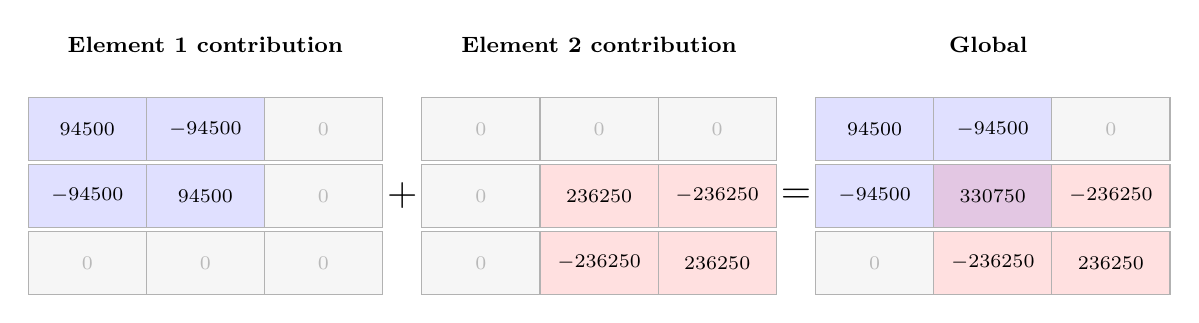
\begin{tikzpicture}[
    cell/.style={draw=gray!60, minimum width=15mm, minimum height=8mm,
                 inner sep=0pt, anchor=center, font=\scriptsize, align=center},
    e1/.style={cell, fill=blue!12},
    e2/.style={cell, fill=red!12},
    e12/.style={cell, fill=violet!22},
    zc/.style={cell, fill=gray!7, text=gray!55},
    title/.style={font=\bfseries\footnotesize, anchor=south}]
  %% Matrix 1: element 1 contribution
  \node[title] at (1.5,1.7) {Element~1 contribution};
  \node[e1] at (0.0,0.85) {$94500$};
  \node[e1] at (1.5,0.85) {$-94500$};
  \node[zc]  at (3.0,0.85) {$0$};
  \node[e1] at (0.0,0.00) {$-94500$};
  \node[e1] at (1.5,0.00) {$94500$};
  \node[zc]  at (3.0,0.00) {$0$};
  \node[zc]  at (0.0,-0.85) {$0$};
  \node[zc]  at (1.5,-0.85) {$0$};
  \node[zc]  at (3.0,-0.85) {$0$};
  %% Plus
  \node[font=\Large\bfseries] at (4.0,0) {$+$};
  %% Matrix 2: element 2 contribution
  \node[title] at (6.5,1.7) {Element~2 contribution};
  \node[zc]  at (5.0,0.85) {$0$};
  \node[zc]  at (6.5,0.85) {$0$};
  \node[zc]  at (8.0,0.85) {$0$};
  \node[zc]  at (5.0,0.00) {$0$};
  \node[e2] at (6.5,0.00) {$236250$};
  \node[e2] at (8.0,0.00) {$-236250$};
  \node[zc]  at (5.0,-0.85) {$0$};
  \node[e2] at (6.5,-0.85) {$-236250$};
  \node[e2] at (8.0,-0.85) {$236250$};
  %% Equals
  \node[font=\Large\bfseries] at (9.0,0) {$=$};
  %% Matrix 3: assembled global K
  \node[title] at (11.5,1.7) {Global $\stiff$};
  \node[e1]  at (10.0,0.85) {$94500$};
  \node[e1]  at (11.5,0.85) {$-94500$};
  \node[zc]   at (13.0,0.85) {$0$};
  \node[e1]  at (10.0,0.00) {$-94500$};
  \node[e12] at (11.5,0.00) {$330750$};
  \node[e2]  at (13.0,0.00) {$-236250$};
  \node[zc]   at (10.0,-0.85) {$0$};
  \node[e2]  at (11.5,-0.85) {$-236250$};
  \node[e2]  at (13.0,-0.85) {$236250$};
\end{tikzpicture}
\caption{Graphical assembly of the global stiffness matrix. Blue cells receive contributions from element~1, red cells from element~2, and the violet cell at row/column~2 receives contributions from both, giving $94{,}500 + 236{,}250 = 330{,}750$.}
\label{fig:stepped_bar_K_assembly}
\end{figure}

\paragraph{Force vector assembly.}
The distributed-load contribution from element~1 lands at DOFs 1 and 2; the
concentrated forces are placed directly at their respective nodes:
\[
   \vect{f}_p = \begin{bmatrix} -1000 \\ -1000 \\ 0 \end{bmatrix},\quad
   \vect{f}_c = \begin{bmatrix} 0 \\ 6000 \\ -15000 \end{bmatrix},\quad
   \vect{f} = \vect{f}_p + \vect{f}_c
            = \begin{bmatrix} -1000 \\ 5000 \\ -15000 \end{bmatrix}\,\text{N} .
\]

\paragraph{Boundary conditions and reduced system.}
Node~1 is fixed, $u_1 = 0$. The free-DOF set is $\{2,3\}$. Striking the first
row and column,
\[
   \underbrace{\begin{bmatrix} 330{,}750 & -236{,}250 \\ -236{,}250 & 236{,}250 \end{bmatrix}}_{\stiff_{ff}}
   \begin{bmatrix} u_2 \\ u_3 \end{bmatrix}
   =
   \underbrace{\begin{bmatrix} 5{,}000 \\ -15{,}000 \end{bmatrix}}_{\vect{f}_f} .
\]
Solving,
\[
   u_2 = -\tfrac{20}{189} \approx -0.1058 \;\text{mm},
   \qquad
   u_3 = -\tfrac{32}{189} \approx -0.1693 \;\text{mm}.
\]

\paragraph{Reaction at the fixed support.}
The reaction follows from the first row of the unreduced system:
\[
   R_1 = \stiff_{1,*}\,\vect{u} - f_1
       = (-94{,}500)(-\tfrac{20}{189}) - (-1000) = +11{,}000 \;\text{N},
\]
which balances the resultant of all applied axial forces:
$-(-2000) - 6000 - (-15000) = +11{,}000$~N.

\paragraph{Internal displacement and force fields.}
Inside each element the displacement follows the enriched trial
\cref{eq:bar_disp_enriched}, evaluated with the nodal solution and the
particular solution \cref{eq:up_uniform}. Differentiating yields
$N(x)$ from \cref{eq:bar_force_enriched}. The resulting curves
(\cref{fig:stepped_bar_u,fig:stepped_bar_N}) show the parabolic curvature in
element~1 caused by $p_1 \neq 0$, the linear field in element~2, and the
$+6$~kN jump in $N(x)$ at $x = 500$~mm corresponding to the concentrated load
applied there.

\begin{figure}[htbp]
\centering
\includegraphics[width=0.85\textwidth]{figures/stepped_bar_displacement.pdf}
\caption{Displacement field $u(x)$ along the stepped bar.}
\label{fig:stepped_bar_u}
\end{figure}

\begin{figure}[htbp]
\centering
\includegraphics[width=0.85\textwidth]{figures/stepped_bar_internal_force.pdf}
\caption{Internal axial force $N(x)$ along the stepped bar. The discontinuity at $x = 500$~mm corresponds to the $+6$~kN concentrated force applied at node~2.}
\label{fig:stepped_bar_N}
\end{figure}

\noindent See \Cref{lst:stepped_bar} in the Appendix for the full MATLAB
implementation that produced these plots.
\end{example}

\section{Principle of Virtual Work for the Axial Bar}
\label{sec:pvw}

The direct formulation of \cref{sec:direct_formulation} and the worked
examples above gave the bar element stiffness and load vector from physical
equilibrium. The principle of virtual work (PVW) provides an alternative,
energy-based statement of equilibrium that reproduces the same results and
generalizes immediately to non-uniform loading, variable cross-section, and
higher-order elements. PVW is the variational foundation on which the entire
finite element method rests.

\subsection{Statement of the Principle}

\begin{importantbox}
\textbf{Principle of Virtual Work:}
For a bar in static equilibrium, and for any \emph{kinematically admissible}
virtual displacement field $\delta u(x)$,
\begin{equation}
    \delta W_{\mathrm{int}} = \delta W_{\mathrm{ext}} ,
    \label{eq:pvw_statement}
\end{equation}
with internal and external virtual work
\[
   \delta W_{\mathrm{int}}
     = \int_0^L N(x)\,\delta\varepsilon(x)\,\dd x
     = \int_0^L EA\,\frac{\dd u}{\dd x}\,\frac{\dd \delta u}{\dd x}\,\dd x ,
\]
\[
   \delta W_{\mathrm{ext}}
     = \int_0^L p(x)\,\delta u(x)\,\dd x
     + \sum_i F_i\,\delta u(x_i) .
\]
A virtual displacement is \emph{kinematically admissible} if it satisfies the
essential boundary conditions: $\delta u = 0$ wherever $u$ is prescribed.
\end{importantbox}

The virtual displacement $\delta u(x)$ is an arbitrary, infinitesimal
perturbation. It need not satisfy equilibrium or any natural boundary
conditions — its sole role is to test the equilibrium of the actual
displacement field $u(x)$.

\subsection{Derivation from Equilibrium}

Begin with the local equilibrium equation derived in
\cref{ch:weighted_residuals}:
\begin{equation}
    \frac{\dd N}{\dd x} + p(x) = 0, \qquad 0 < x < L .
    \label{eq:pvw_equilibrium}
\end{equation}
Multiply both sides by an arbitrary virtual displacement $\delta u(x)$ and
integrate over the bar:
\begin{equation}
    \int_0^L \left( \frac{\dd N}{\dd x} + p \right) \delta u\,\dd x = 0 .
    \label{eq:pvw_integral}
\end{equation}
Integration by parts on the first term gives
\begin{equation}
    \int_0^L \frac{\dd N}{\dd x}\,\delta u\,\dd x
    = \big[N(x)\,\delta u(x)\big]_0^L
    - \int_0^L N(x)\,\frac{\dd \delta u}{\dd x}\,\dd x .
    \label{eq:pvw_ibp}
\end{equation}
Substituting back into \cref{eq:pvw_integral} and rearranging,
\begin{equation}
    \int_0^L N\,\frac{\dd \delta u}{\dd x}\,\dd x
    = \big[N\,\delta u\big]_0^L + \int_0^L p\,\delta u\,\dd x .
    \label{eq:pvw_weak}
\end{equation}
The boundary term vanishes wherever the displacement is prescribed (kinematic
admissibility forces $\delta u = 0$ there) and reduces to $F_i\,\delta u(x_i)$
at any free end with a concentrated force $F_i$ (because $N$ at that end
equals the applied force). Substituting the constitutive law
$N = EA\,\dd u/\dd x$ and $\delta\varepsilon = \dd \delta u/\dd x$ on the
left, equation \cref{eq:pvw_weak} becomes
\begin{equation}
    \int_0^L EA\,\frac{\dd u}{\dd x}\,\frac{\dd \delta u}{\dd x}\,\dd x
    \;=\;
    \int_0^L p\,\delta u\,\dd x \;+\; \sum_i F_i\,\delta u(x_i) ,
    \label{eq:pvw_final}
\end{equation}
which is exactly the PVW statement \cref{eq:pvw_statement}.

\begin{remark}
Equation \cref{eq:pvw_final} is the \emph{weak form} of the bar equilibrium
equation. The strong form $-EA\,u'' = p$ requires twice-differentiable trial
functions; the weak form requires only first derivatives. This relaxation
makes the weak form well-suited to piecewise-polynomial finite element
approximations whose derivatives may be discontinuous between elements.
\end{remark}

\subsection{Recovery of the Bar Stiffness Matrix}

To reproduce the element stiffness derived in \cref{sec:direct_formulation},
substitute the linear interpolation
\begin{equation}
    u(x) = N_1(x)\,u_1 + N_2(x)\,u_2,
    \qquad
    \delta u(x) = N_1(x)\,\delta u_1 + N_2(x)\,\delta u_2 ,
\end{equation}
with strain-displacement matrix $\matr{B} = \tfrac{1}{L}[\,-1,\;1\,]$, into
the left-hand side of \cref{eq:pvw_final}:
\[
    \delta \vect{u}^{e\transpose}\!
    \left[\int_0^L EA\,\matr{B}\transpose \matr{B}\,\dd x\right]
    \!\vect{u}^e
    = \delta \vect{u}^{e\transpose}\,\matr{k}^e\,\vect{u}^e ,
\]
giving
\[
    \matr{k}^e
    = \int_0^L EA\,\matr{B}\transpose \matr{B}\,\dd x
    = \frac{EA}{L}\begin{bmatrix} 1 & -1 \\ -1 & 1 \end{bmatrix} ,
\]
identical to \cref{eq:bar_stiffness}. The right-hand side likewise produces
the consistent load vector $\vect{f}^e = \int_0^L \vect{N}\transpose p\,\dd x +
(\text{nodal forces})$. Direct mechanics, weak form, and PVW all give the same
element equations.

\subsection{Worked Example: Verification of PVW on the Stepped Bar}
\label{sec:pvw_verification}

\begin{example}[Numerical verification of $\delta W_{\mathrm{int}} = \delta W_{\mathrm{ext}}$]
\label{ex:pvw_verification}

To illustrate that PVW holds for a real loaded bar in equilibrium, we
return to the stepped bar of \cref{ex:stepped_bar} (already solved
exactly). Recall the actual nodal solution
\[
   u_1 = 0,\quad
   u_2 = -\tfrac{20}{189} \approx -0.10582 \;\text{mm},\quad
   u_3 = -\tfrac{32}{189} \approx -0.16931 \;\text{mm},
\]
the support reaction $R_1 = +11{,}000$~N, and the internal axial force per
element from \cref{eq:bar_force_enriched},
\begin{align*}
   N^{(1)}(x_1) &= \tfrac{EA_1(u_2-u_1)}{L_1} + \tfrac{p_1(L_1-2x_1)}{2}
                = -10{,}000 + (-2)(500-2x_1)
                = -11{,}000 + 4x_1 \;\;[\text{N}], \\
   N^{(2)}(x_2) &= \tfrac{EA_2(u_3-u_2)}{L_2}
                = -15{,}000 \;\;[\text{N}] \quad (\text{constant}),
\end{align*}
where $x_1 \in [0,500]$ and $x_2 \in [0,400]$ are local element coordinates.

We now choose two different kinematically admissible virtual displacements
$\delta u(x)$ (each must satisfy $\delta u(0)=0$) and verify the equality
$\delta W_{\mathrm{int}} = \delta W_{\mathrm{ext}}$ by direct calculation
of both sides.

\paragraph{Case A: $(\delta u_1,\delta u_2,\delta u_3) = (0,1,0)$ ``tent''.}

Piecewise linear with the apex at node 2:
\[
   \delta u^{(1)}(x_1) = \frac{x_1}{L_1} = \frac{x_1}{500}, \qquad
   \delta u^{(2)}(x_2) = 1 - \frac{x_2}{L_2} = 1 - \frac{x_2}{400} .
\]
The corresponding virtual strains are constant on each element:
\[
   \delta\varepsilon^{(1)} = +\tfrac{1}{500}, \qquad
   \delta\varepsilon^{(2)} = -\tfrac{1}{400} .
\]

\noindent\emph{Internal virtual work.}
For an element with constant $EA$ and uniform $p$, $\int_0^{L} N(x)\,\dd x =
EA(u_b - u_a)$ (the distributed-load contribution integrates to zero). Hence
\begin{align*}
   \delta W_{\mathrm{int}}^{(1)}
   &= \delta\varepsilon^{(1)}\!\int_0^{L_1}\! N^{(1)}\,\dd x_1
    = \tfrac{1}{500}\,EA_1(u_2-u_1)
    = \tfrac{1}{500}\,(-5{,}000{,}000) = -10{,}000\;\text{N\,mm}, \\
   \delta W_{\mathrm{int}}^{(2)}
   &= \delta\varepsilon^{(2)}\!\int_0^{L_2}\! N^{(2)}\,\dd x_2
    = -\tfrac{1}{400}\,EA_2(u_3-u_2)
    = -\tfrac{1}{400}\,(-6{,}000{,}000) = +15{,}000\;\text{N\,mm}, \\
   \delta W_{\mathrm{int}}
   &= -10{,}000 + 15{,}000 = +5{,}000 \;\text{N\,mm}.
\end{align*}

\noindent\emph{External virtual work.}
The reaction at node~1 does no virtual work because $\delta u_1 = 0$.
\begin{align*}
   \int_0^{L_1}\! p_1\,\delta u^{(1)}\,\dd x_1
   &= \int_0^{500}\!(-4)\!\left(\tfrac{x_1}{500}\right)\!\dd x_1
    = -1{,}000\;\text{N\,mm}, \\
   F_2\,\delta u_2 + F_3\,\delta u_3
   &= (6{,}000)(1) + (-15{,}000)(0) = +6{,}000\;\text{N\,mm}, \\
   \delta W_{\mathrm{ext}}
   &= -1{,}000 + 6{,}000 = +5{,}000 \;\text{N\,mm}.
\end{align*}

\noindent\textbf{Result:} $\delta W_{\mathrm{int}} = \delta W_{\mathrm{ext}} = +5{,}000$~N\,mm. \hfill\checkmark

\paragraph{Case B: $(\delta u_1,\delta u_2,\delta u_3) = (0,1,1)$ ``ramp''.}

Linear in element~1, constant in element~2:
\[
   \delta u^{(1)} = \frac{x_1}{500},\qquad \delta u^{(2)} = 1,
   \qquad
   \delta\varepsilon^{(1)} = \tfrac{1}{500},\qquad \delta\varepsilon^{(2)} = 0 .
\]
\begin{align*}
   \delta W_{\mathrm{int}}
   &= \tfrac{1}{500}(-5{,}000{,}000) + 0 = -10{,}000\;\text{N\,mm}, \\
   \delta W_{\mathrm{ext}}
   &= \underbrace{-1{,}000}_{\text{distributed load}}
    + \underbrace{(6{,}000)(1) + (-15{,}000)(1)}_{\text{concentrated forces}}
    = -1{,}000 - 9{,}000 = -10{,}000\;\text{N\,mm}.
\end{align*}
\textbf{Result:} $\delta W_{\mathrm{int}} = \delta W_{\mathrm{ext}} = -10{,}000$~N\,mm. \hfill\checkmark

\medskip

The two virtual displacements above coincide with the basis used in the FEM
discretization (piecewise linear, one unit value at a free DOF, zero
elsewhere). Choosing $\delta u$ as the $i$-th basis function reproduces
exactly the $i$-th row of the reduced FEM equations $\stiff_{ff}\vect{u}_f =
\vect{f}_f$. Indeed, $+5{,}000$ and $-10{,}000$ are the assembled effective
forces at DOF~2 and DOF~$2{+}3$ for these two perturbations.

\paragraph{Beyond piecewise linear.}
PVW holds for any kinematically admissible virtual displacement, not just
those built from the FEM basis. The MATLAB script
\Cref{lst:pvw_verification} also evaluates a smooth quadratic
$\delta u(x) = (x/900)^2$ and reports
\[
   \delta W_{\mathrm{int}} = \delta W_{\mathrm{ext}} \approx -13{,}353.91 \;\text{N\,mm}
   \qquad (|\Delta| < 10^{-11}\;\text{N\,mm}) ,
\]
confirming that the work balance is independent of the chosen test field.

\begin{remark}
This verification is more than a numerical check — it is the defining property
of the equilibrium configuration. Of all kinematically admissible
displacement fields, the actual $u(x)$ is the unique one for which the work
balance holds for \emph{every} admissible perturbation. The finite element
method exploits this property: by enforcing PVW with the basis functions of
the chosen mesh as test fields, it produces the discrete equations
$\stiff\vect{u} = \vect{f}$ whose solution is the best approximation to the
true equilibrium within that finite-dimensional space.
\end{remark}

\end{example}

% =============================================================================
\section{Galerkin Finite Element Formulation of the Bar}
\label{sec:galerkin_fe}
% =============================================================================

\begin{remark}
\Cref{ch:weighted_residuals} applied the Galerkin method with a single global
polynomial -- one free parameter, one weight function -- to the continuous bar.
The formulation developed here uses the finite element shape functions $N_1$,
$N_2$ of \cref{eq:bar_shape} as both trial and test functions on each element.
With piecewise-linear shape functions and one test function per node, this is
the Galerkin principle applied at the element level: the method through which
every finite element stiffness integral is derived in practice.
\end{remark}

\subsection{From Weighted Residuals to Shape Functions}
\label{sec:galerkin_fe_intro}

Start from the strong form of the loaded bar (\cref{eq:bar_de}):
\[
    -EA\,\frac{\dd^2 u}{\dd x^2} = p(x), \qquad 0 < x < L .
\]
Substitute the finite element approximation $u^h(x) = \vect{N}(x)\,\vect{u}^e$
from \cref{eq:bar_disp}. Because $N_1$ and $N_2$ are linear in $x$, their
second derivative vanishes identically, so the residual is
\begin{equation}
    R(x) = -EA\,\frac{\dd^2 u^h}{\dd x^2} - p(x) = -p(x) \neq 0 .
    \label{eq:galerkin_fe_residual}
\end{equation}
The linear approximation cannot satisfy the ODE pointwise when $p(x) \neq 0$;
it satisfies it instead in an \emph{average} sense. The \textbf{Galerkin
statement} requires the residual to be orthogonal to each shape function:
\begin{equation}
    \int_0^L N_i(x)\,R(x)\,\dd x = 0, \qquad i = 1,\,2 .
    \label{eq:galerkin_fe_statement}
\end{equation}
This choice -- test functions identical to the trial functions -- is called the
\emph{Bubnov--Galerkin} method and is standard for self-adjoint problems such
as linear elasticity.

\subsection{Galerkin Weak Form for a Single Element}
\label{sec:galerkin_fe_weak}

Substituting \cref{eq:galerkin_fe_residual} into \cref{eq:galerkin_fe_statement}
and expanding:
\[
    \int_0^L N_i\!\left(-EA\,\frac{\dd^2 u^h}{\dd x^2} - p\right)\dd x = 0 .
\]
Integration by parts on the second-derivative term (the same step as
\cref{eq:pvw_ibp}) gives
\begin{equation}
    \int_0^L EA\,\frac{\dd N_i}{\dd x}\,\frac{\dd u^h}{\dd x}\,\dd x
    \;-\;
    \Bigl[N_i\,EA\,\frac{\dd u^h}{\dd x}\Bigr]_0^L
    \;=\;
    \int_0^L N_i\,p\,\dd x .
    \label{eq:galerkin_fe_ibp}
\end{equation}
The boundary term vanishes at nodes where the displacement is prescribed
(kinematic admissibility requires $N_i = 0$ there), and reduces to the applied
concentrated force $F$ at a free end via the natural boundary condition
$EA\,\dd u/\dd x = F$. The result is the \textbf{Galerkin weak form}:
\begin{equation}
    \int_0^L EA\,\frac{\dd N_i}{\dd x}\,\frac{\dd u^h}{\dd x}\,\dd x
    \;=\;
    \int_0^L N_i\,p\,\dd x \;+\; F_i^{\mathrm{natural}} .
    \label{eq:galerkin_fe_weak_i}
\end{equation}

\subsection{Element Stiffness Matrix and Load Vector}
\label{sec:galerkin_fe_matrices}

Writing both rows ($i = 1$ and $i = 2$) simultaneously in matrix form,
\[
    \underbrace{
    \left[\int_0^L EA\,\matr{B}\transpose\matr{B}\,\dd x\right]
    }_{\matr{k}^e}\!\vect{u}^e
    \;=\;
    \underbrace{
    \int_0^L \vect{N}\transpose p\,\dd x
    }_{\vect{f}^e} ,
\]
where $\matr{B} = \dd\vect{N}/\dd x = \tfrac{1}{L}[\,-1,\;1\,]$ from
\cref{eq:bar_strain}. Evaluating the integrals:
\begin{align}
    \matr{k}^e
    &= \int_0^L EA\,\matr{B}\transpose\matr{B}\,\dd x
     = \frac{EA}{L}\begin{bmatrix}1&-1\\-1&1\end{bmatrix} ,
    \label{eq:galerkin_fe_ke_integral} \\[4pt]
    \vect{f}^e
    &= \int_0^L \vect{N}\transpose p_0\,\dd x
     = p_0\int_0^L\begin{bmatrix}1-x/L\\x/L\end{bmatrix}\dd x
     = \frac{p_0 L}{2}\begin{bmatrix}1\\1\end{bmatrix} ,
    \label{eq:galerkin_fe_fe_integral}
\end{align}
in exact agreement with \cref{eq:bar_stiffness} and \cref{eq:bar_load}.

\begin{importantbox}
The Galerkin finite element formulation yields
\[
    \matr{k}^e = \int_0^L EA\,\matr{B}\transpose\matr{B}\,\dd x
              = \frac{EA}{L}\begin{bmatrix}1&-1\\-1&1\end{bmatrix},
    \qquad
    \vect{f}^e = \int_0^L \vect{N}\transpose p\,\dd x
              = \frac{p_0 L}{2}\begin{bmatrix}1\\1\end{bmatrix},
\]
identical to \cref{eq:bar_stiffness} and \cref{eq:bar_load}.
\end{importantbox}

% =============================================================================
\section{Equivalence of Galerkin and Virtual Work Formulations}
\label{sec:galerkin_pvw_equivalence}
% =============================================================================

The Galerkin weak form \cref{eq:galerkin_fe_weak_i} and the PVW equation
\cref{eq:pvw_final} are the same integral statement. To see this, write them
side by side:
\begin{align}
    \text{PVW:}\quad
    &\int_0^L EA\,\frac{\dd u}{\dd x}\,\frac{\dd\delta u}{\dd x}\,\dd x
     = \int_0^L p\,\delta u\,\dd x + \sum_i F_i\,\delta u(x_i) , \notag \\[4pt]
    \text{Galerkin FE:}\quad
    &\int_0^L EA\,\frac{\dd u^h}{\dd x}\,\frac{\dd w_i}{\dd x}\,\dd x
     = \int_0^L p\,w_i\,\dd x + \sum_i F_i\,w_i(x_i) .
    \label{eq:galerkin_pvw_comparison}
\end{align}
Setting $w_i = \delta u$, the two expressions are identical: both require the
integral to vanish for every kinematically admissible test field, and both
produce the same discrete system $\matr{k}^e\,\vect{u}^e = \vect{f}^e$.

\begin{remark}
PVW speaks the language of mechanics: $\delta u$ is an infinitesimal virtual
displacement, and the equation expresses the balance of virtual internal and
external work. Galerkin speaks the language of weighted residuals: $w_i = N_i$
is a test function chosen to make the residual orthogonal to the approximation
space. They are the same mathematical object. In the finite element context,
both methods mandate choosing test functions from the same polynomial space as
the trial -- which is why they produce identical element matrices.
\end{remark}

% =============================================================================
\section{Principle of Minimum Potential Energy}
\label{sec:pmpe}
% =============================================================================

\subsection{Total Potential Energy of the Axial Bar}
\label{sec:pmpe_tpe}

\begin{definition}
The \textbf{strain energy} stored in a linearly elastic axially loaded bar is
\begin{equation}
    U = \frac{1}{2}\int_0^L EA\!\left(\frac{\dd u}{\dd x}\right)^{\!2}\dd x .
    \label{eq:pmpe_strain_energy}
\end{equation}
The \textbf{total potential energy} is
\begin{equation}
    \Pi[u] = U - W_{\mathrm{ext}},
    \qquad
    W_{\mathrm{ext}} = \int_0^L p(x)\,u(x)\,\dd x + \sum_i F_i\,u(x_i) .
    \label{eq:pmpe_tpe}
\end{equation}
\end{definition}

\noindent
The strain energy $U \geq 0$ is always non-negative. The total potential energy
$\Pi$ is a functional of the displacement field $u(x)$: each admissible $u$
gives a scalar value of $\Pi$, and the equilibrium field is singled out by a
stationarity condition.

\subsection{Stationarity Condition and the Weak Form}
\label{sec:pmpe_stationarity}

\begin{importantbox}
\textbf{Principle of Minimum Potential Energy (PMPE):} Of all kinematically
admissible displacement fields, the one that satisfies equilibrium makes the
total potential energy stationary:
\begin{equation}
    \delta\Pi = 0
\end{equation}
for every admissible variation $\delta u$. For a stable elastic equilibrium,
$\Pi$ is in fact a global minimum.
\end{importantbox}

Taking the first variation of \cref{eq:pmpe_tpe},
\begin{equation}
    \delta\Pi
    = \int_0^L EA\,\frac{\dd u}{\dd x}\,\frac{\dd\delta u}{\dd x}\,\dd x
      \;-\;
      \int_0^L p\,\delta u\,\dd x
      \;-\;
      \sum_i F_i\,\delta u(x_i)
      \;=\; 0 .
    \label{eq:pmpe_first_variation}
\end{equation}
Recognizing the first integral as $\delta W_{\mathrm{int}}$ and the remaining
terms as $\delta W_{\mathrm{ext}}$, this is precisely the PVW statement
\cref{eq:pvw_statement}:
\begin{equation}
    \delta\Pi = 0
    \;\Longleftrightarrow\;
    \delta W_{\mathrm{int}} = \delta W_{\mathrm{ext}} .
    \label{eq:pmpe_pvw_link}
\end{equation}

\begin{remark}
PMPE is a special case of PVW valid for \emph{conservative} systems, where the
material is linearly elastic and the external loads are independent of the
deformation. For the axially loaded bar with fixed applied loads, the two
principles are exactly equivalent. PVW is the more general statement: it
extends to non-conservative loading (e.g.\ follower loads) for which no
potential energy exists.
\end{remark}

\subsection{Element Stiffness Matrix and Load Vector from PMPE}
\label{sec:pmpe_matrices}

Substitute the finite element trial $u = \vect{N}\,\vect{u}^e$,
$\dd u/\dd x = \matr{B}\,\vect{u}^e$ into the element contributions to
\cref{eq:pmpe_tpe}. The strain energy becomes
\[
    U^e = \frac{1}{2}\int_0^L EA\,\vect{u}^{e\transpose}\matr{B}\transpose\matr{B}\,\vect{u}^e\,\dd x
        = \frac{1}{2}\,\vect{u}^{e\transpose}
          \!\underbrace{\left[\int_0^L EA\,\matr{B}\transpose\matr{B}\,\dd x\right]}_{\matr{k}^e}
          \!\vect{u}^e
        = \frac{1}{2}\,\vect{u}^{e\transpose}\matr{k}^e\,\vect{u}^e ,
\]
and the work of external loads (uniform $p_0$):
\[
    W_{\mathrm{ext}}^e = \int_0^L (\vect{N}\,\vect{u}^e)\,p_0\,\dd x
        = \vect{u}^{e\transpose}
          \!\underbrace{\left[\int_0^L \vect{N}\transpose p_0\,\dd x\right]}_{\vect{f}^e}
        = \vect{u}^{e\transpose}\vect{f}^e .
\]
The element potential energy is therefore a quadratic function of the nodal
displacements:
\begin{equation}
    \Pi^e = \frac{1}{2}\,\vect{u}^{e\transpose}\matr{k}^e\,\vect{u}^e
            - \vect{u}^{e\transpose}\vect{f}^e .
    \label{eq:pmpe_tpe_element}
\end{equation}
Differentiating with respect to $\vect{u}^e$ and setting the result to zero,
\begin{equation}
    \frac{\partial\Pi^e}{\partial\vect{u}^e}
    = \matr{k}^e\,\vect{u}^e - \vect{f}^e = \vect{0}
    \quad\Longrightarrow\quad
    \matr{k}^e\,\vect{u}^e = \vect{f}^e .
    \label{eq:pmpe_stationarity_result}
\end{equation}
The integrals evaluate to \cref{eq:galerkin_fe_ke_integral} and
\cref{eq:galerkin_fe_fe_integral}, so $\matr{k}^e$ and $\vect{f}^e$ are again
identical to \cref{eq:bar_stiffness} and \cref{eq:bar_load}.

\begin{importantbox}
Minimizing the element potential energy yields
\[
    \matr{k}^e
    = \int_0^L EA\,\matr{B}\transpose\matr{B}\,\dd x
    = \frac{EA}{L}\begin{bmatrix}1&-1\\-1&1\end{bmatrix} .
\]
The stiffness matrix is the Hessian of the strain energy with respect to the
nodal displacements.
\end{importantbox}

\subsection{Summary: Four Equivalent Paths to the Same Element Matrices}
\label{sec:pmpe_summary}

Four independent derivations all produce the same element stiffness matrix
$\matr{k}^e$ (\cref{eq:bar_stiffness}) and load vector $\vect{f}^e$
(\cref{eq:bar_load}).

\begin{table}[htbp]
\centering
\small
\caption{Four derivation paths for the bar element matrices.}
\label{tab:four_methods}
\begin{tabular}{@{}lp{2.8cm}p{3.8cm}p{3.6cm}@{}}
\toprule
\textbf{Method}
  & \textbf{Starting point}
  & \textbf{Path to $\matr{k}^e$}
  & \textbf{Load vector $\vect{f}^e$} \\
\midrule
Direct Equilibrium
  & Hooke's law $+$ nodal force balance
  & $N = EA\varepsilon$; collect into matrix form
  & Enriched trial $+$ end reactions (\cref{sec:displacement_field}) \\[6pt]
PVW
  & $\delta W_{\mathrm{int}} = \delta W_{\mathrm{ext}}$ (\cref{eq:pvw_statement})
  & Substitute $u = \vect{N}\vect{u}^e$, $\delta u = \vect{N}\delta\vect{u}^e$
  & RHS of weak form (\cref{sec:pvw}) \\[6pt]
Galerkin FE
  & $\int N_i R\,\dd x = 0$,\newline $w_i = N_i$ (\cref{eq:galerkin_fe_statement})
  & Integration by parts $+$ $\matr{B}$-matrix (\cref{sec:galerkin_fe})
  & RHS of weak form (\cref{eq:galerkin_fe_fe_integral}) \\[6pt]
PMPE
  & $\delta\Pi = 0$, $\Pi = U - W_{\mathrm{ext}}$ (\cref{eq:pmpe_tpe})
  & Substitute FE trial into $U^e$; stationarity $\partial\Pi^e/\partial\vect{u}^e = \vect{0}$
  & $\partial W_{\mathrm{ext}}^e/\partial\vect{u}^e$ (\cref{sec:pmpe_matrices}) \\
\bottomrule
\end{tabular}
\end{table}

The choice of method is a matter of convenience and generalizability. Direct
equilibrium is intuitive for one-dimensional elements. PVW and Galerkin FE
extend unchanged to two- and three-dimensional elements
(\cref{ch:2d_continuum}); PMPE extends to any conservative system. Numerically,
all four paths lead to the same linear system $\stiff\,\vect{u} = \vect{f}$,
as confirmed by the MATLAB scripts \Cref{lst:pvw_verification} and
\Cref{lst:stepped_bar}.

\section{Natural Coordinates and Isoparametric Mapping}
\label{sec:isoparametric_1d}

The element formulations developed so far were written directly in the
physical coordinate $x \in [0, L]$. For higher-order elements, distorted
geometries, and two- or three-dimensional continua, it is far more
convenient to work in a fixed \emph{natural} (or \emph{parametric})
coordinate $\xi \in [-1, 1]$, the same for every element regardless of its
size or position. The mapping between $\xi$ and $x$ is built from the same
shape functions used to interpolate the displacement --- the defining
property of the \emph{isoparametric} concept. We now re-derive the bar
element matrices in this framework and recover the familiar results
\cref{eq:bar_stiffness} and \cref{eq:bar_load}.

\subsection{The Isoparametric Mapping}

Define the linear coordinate transformation
\begin{equation}
    x(\xi) = N_1(\xi)\, x_1 + N_2(\xi)\, x_2
    = \frac{1-\xi}{2}\, x_1 + \frac{1+\xi}{2}\, x_2,
    \qquad \xi \in [-1,1],
    \label{eq:isomap_1d}
\end{equation}
which sends $\xi = -1 \mapsto x = x_1$ and $\xi = +1 \mapsto x = x_2$. The
shape functions in natural coordinates are
\begin{equation}
    N_1(\xi) = \frac{1-\xi}{2}, \qquad N_2(\xi) = \frac{1+\xi}{2},
    \label{eq:bar_shape_xi}
\end{equation}
and they satisfy $N_i(\xi_j) = \delta_{ij}$ at the parent nodes
$\xi_1 = -1$, $\xi_2 = +1$, together with the partition of unity
$N_1(\xi) + N_2(\xi) = 1$.

The displacement is interpolated with the \emph{same} two functions,
\begin{equation}
    u(\xi) = N_1(\xi)\, u_1 + N_2(\xi)\, u_2
    = \vect{N}(\xi)\,\vect{u}^e,
    \label{eq:bar_disp_xi}
\end{equation}
which is what makes the formulation isoparametric: a single set of
$\{N_i(\xi)\}$ describes both the geometry and the field.

\subsection{Jacobian of the Mapping}

The Jacobian of \cref{eq:isomap_1d} measures how a unit length in the
parent domain stretches into the physical domain:
\begin{equation}
    J(\xi) = \frac{\dd x}{\dd\xi}
    = \sum_{i=1}^{2} \frac{\dd N_i}{\dd\xi}\, x_i
    = -\tfrac{1}{2}\, x_1 + \tfrac{1}{2}\, x_2
    = \frac{x_2 - x_1}{2} = \frac{L}{2}.
    \label{eq:jacobian_1d}
\end{equation}
For the two-node linear bar the Jacobian is \emph{constant} and equal to
half the element length. The differential transforms as
$\dd x = J\,\dd\xi = (L/2)\,\dd\xi$, and the inverse Jacobian needed for
the chain rule is $J^{-1} = 2/L$.

\begin{remark}
$J(\xi)$ being constant is a special feature of the linear 1D element on
a uniform mesh. For curved sides (Q4 in \cref{ch:2d_continuum}) or
higher-order shape functions, $J$ varies over the element and the
integrals below can no longer be evaluated by inspection.
\end{remark}

\subsection{Strain-Displacement Matrix in Natural Coordinates}

The strain $\varepsilon = \dd u/\dd x$ requires a derivative with respect
to $x$, while $u$ is now a function of $\xi$. The chain rule supplies the
missing factor:
\begin{equation}
    \varepsilon
    = \frac{\dd u}{\dd x}
    = \frac{\dd u}{\dd\xi}\frac{\dd\xi}{\dd x}
    = J^{-1}\,\frac{\dd u}{\dd\xi}
    = \frac{2}{L}\,\frac{\dd u}{\dd\xi}.
\end{equation}
Substituting \cref{eq:bar_disp_xi}, $\dd u/\dd\xi
= -\tfrac{1}{2}\,u_1 + \tfrac{1}{2}\,u_2$, gives
\begin{equation}
    \varepsilon(\xi) = \matr{B}(\xi)\,\vect{u}^e,
    \qquad
    \matr{B}(\xi) = J^{-1}\frac{\dd \vect{N}}{\dd\xi}
    = \frac{2}{L}\,\tfrac{1}{2}\begin{bmatrix} -1 & 1 \end{bmatrix}
    = \frac{1}{L}\begin{bmatrix} -1 & 1 \end{bmatrix} ,
    \label{eq:bar_B_xi}
\end{equation}
which is identical to \cref{eq:bar_strain}. Note that $\matr{B}$ is again
constant in $\xi$: a linear displacement field produces a constant strain,
exactly as in the physical-coordinate derivation.

\subsection{Element Stiffness Matrix via Natural Coordinates}

The element stiffness derived from PVW or Galerkin (\cref{sec:pvw,sec:galerkin_fe}) is
\begin{equation}
    \matr{k}^e = \int_0^{L} \matr{B}\transpose\, EA\, \matr{B} \,\dd x.
\end{equation}
Changing variables to $\xi$ via \cref{eq:isomap_1d}, the limits become
$\pm 1$ and $\dd x = J\,\dd\xi$:
\begin{equation}
    \matr{k}^e = \int_{-1}^{+1} \matr{B}(\xi)\transpose\,EA\,\matr{B}(\xi)
    \, J(\xi)\,\dd\xi .
    \label{eq:ke_natural_1d}
\end{equation}
With $\matr{B}\transpose\matr{B} = (1/L)^2\,[-1\;\;1]\transpose[-1\;\;1]
= (1/L^2)\,\begin{smallmatrix}\phantom{-}1\;\;-1\\-1\;\;\phantom{-}1\end{smallmatrix}$
and $J = L/2$, the integrand is constant:
\begin{equation}
    \matr{B}\transpose EA\,\matr{B}\,J
    = \frac{EA}{L^2}\begin{bmatrix} 1 & -1 \\ -1 & 1 \end{bmatrix}\frac{L}{2}
    = \frac{EA}{2L}\begin{bmatrix} 1 & -1 \\ -1 & 1 \end{bmatrix} .
\end{equation}
Carrying out the trivial integration $\int_{-1}^{+1}\dd\xi = 2$,
\begin{equation}
    \matr{k}^e = \frac{EA}{2L}\begin{bmatrix} 1 & -1 \\ -1 & 1 \end{bmatrix}
                \cdot 2
    = \frac{EA}{L}\begin{bmatrix} 1 & -1 \\ -1 & 1 \end{bmatrix} ,
\end{equation}
recovering \cref{eq:bar_stiffness} exactly.

\subsection{Consistent Load Vector via Natural Coordinates}

For a uniform distributed axial load $p(x) = p_0$, the variational load
vector is $\vect{f}^e = \int_0^L \vect{N}\transpose p \,\dd x$. The same
change of variables produces
\begin{equation}
    \vect{f}^e
    = \int_{-1}^{+1} \vect{N}(\xi)\transpose\, p_0\, J\,\dd\xi
    = p_0\,\frac{L}{2}\!
      \int_{-1}^{+1}\!\!
      \begin{bmatrix} (1-\xi)/2 \\ (1+\xi)/2 \end{bmatrix}\dd\xi .
\end{equation}
Each scalar integral equals one,
\[
    \int_{-1}^{+1}\frac{1-\xi}{2}\,\dd\xi = 1,
    \qquad
    \int_{-1}^{+1}\frac{1+\xi}{2}\,\dd\xi = 1,
\]
so
\begin{equation}
    \vect{f}^e = \frac{p_0 L}{2}\begin{bmatrix} 1 \\ 1 \end{bmatrix} ,
\end{equation}
in agreement with \cref{eq:bar_load}: half of the total distributed load
is lumped at each node, regardless of which coordinate system is used to
evaluate the integral.

\subsection{Numerical Integration: A Preview of Gauss Quadrature}
\label{sec:gauss_preview_1d}

For the bar both integrands above are simple enough to evaluate by hand,
but for higher-order or curved elements they generally cannot be. The
standard remedy is \emph{Gauss--Legendre quadrature}, which approximates
\begin{equation}
    \int_{-1}^{+1} g(\xi)\,\dd\xi \approx \sum_{p=1}^{n_g} w_p\,g(\xi_p),
\end{equation}
with the points $\xi_p$ and weights $w_p$ chosen so that polynomials up
to degree $2n_g - 1$ are integrated \emph{exactly}. For the linear bar:
the integrand of $\matr{k}^e$ is degree~$0$ in $\xi$, and the integrand of
$\vect{f}^e$ is degree~$1$, so a single Gauss point ($n_g = 1$) at
$\xi_1 = 0$ with weight $w_1 = 2$ is already exact.

For the bilinear quadrilateral introduced in \cref{ch:2d_continuum} the
Jacobian is no longer constant, $\matr{B}$ depends on $(\xi,\eta)$, and a
$2\times2$ Gauss rule is required. The structure of the calculation is
nevertheless identical to \cref{eq:ke_natural_1d}: shape functions and
their natural derivatives, a Jacobian, an inverse Jacobian for the
chain rule, and a sum (or integral) over the parent domain. The 1D
derivation in this section is a complete dress rehearsal for that more
general case.

\section{Three-Node Quadratic Rod Element}
\label{sec:bar_3node}

The two-node bar of \cref{sec:isoparametric_1d} carries a linear
displacement field and therefore a constant strain --- adequate for a
uniform $p_0$ on a constant cross-section, but unable to represent the
parabolic displacement that arises whenever the distributed load varies
with $x$ or $EA$ varies along the element. Adding a third node at the
interior of the element produces a \emph{quadratic} (parabolic) bar
element with a linear strain field, a stiffness matrix whose entries can
no longer be evaluated by inspection, and a consistent load vector that
distributes a uniform $p_0$ in the familiar Simpson-rule pattern $1{:}4{:}1$.
This is the simplest non-trivial setting in which to introduce
\emph{Gauss--Legendre numerical integration}, the workhorse of every
isoparametric finite-element code.

\subsection{Quadratic Lagrange Shape Functions}
\label{sec:bar_shape_quad}

Place three nodes at the parent points $\xi_1 = -1$, $\xi_2 = 0$,
$\xi_3 = +1$ and demand that each shape function $N_i(\xi)$ be a
quadratic polynomial satisfying $N_i(\xi_j) = \delta_{ij}$. The unique
solution is the Lagrange triple
\begin{equation}
    N_1(\xi) = \tfrac{1}{2}\xi(\xi-1), \qquad
    N_2(\xi) = 1 - \xi^2, \qquad
    N_3(\xi) = \tfrac{1}{2}\xi(\xi+1) ,
    \label{eq:bar_shape_quad}
\end{equation}
which collectively form a partition of unity, $N_1 + N_2 + N_3 \equiv 1$.
\Cref{fig:bar_shape_quad} plots the three functions on the parent
interval; each rises to unity at its own node and vanishes at the other
two.

\begin{figure}[htbp]
\centering
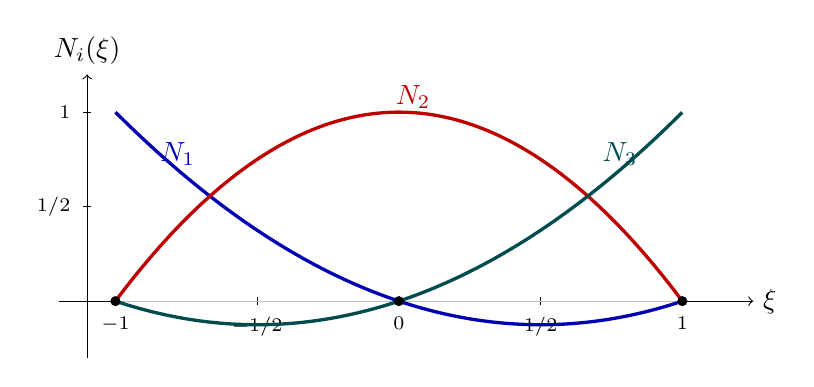
\begin{tikzpicture}[x=3.6cm, y=2.4cm]
  % Axes
  \draw[->] (-1.20,0) -- (1.25,0) node[right] {$\xi$};
  \draw[->] (-1.10,-0.30) -- (-1.10,1.20) node[above] {$N_i(\xi)$};
  % Tick marks on xi-axis
  \foreach \x/\lab in {-1/{-1},-0.5/{-1/2},0/0,0.5/{1/2},1/1} {
      \draw (\x,0.02) -- (\x,-0.02) node[below=1pt] {\scriptsize $\lab$};
  }
  % Tick marks on N-axis
  \foreach \y/\lab in {0.5/{1/2},1/1} {
      \draw (-1.10+0.015,\y) -- (-1.10-0.015,\y) node[left=1pt] {\scriptsize $\lab$};
  }
  % Zero line for clarity
  \draw[gray!50, thin] (-1,0) -- (1,0);
  % N1 = (1/2) xi (xi-1)
  \draw[blue!70!black, very thick, smooth, samples=61, domain=-1:1]
        plot (\x,{0.5*\x*(\x-1)});
  \node[blue!70!black] at (-0.78, 0.78) {$N_1$};
  % N2 = 1 - xi^2
  \draw[red!75!black, very thick, smooth, samples=61, domain=-1:1]
        plot (\x,{1-\x*\x});
  \node[red!75!black] at (0.05, 1.08) {$N_2$};
  % N3 = (1/2) xi (xi+1)
  \draw[teal!60!black, very thick, smooth, samples=61, domain=-1:1]
        plot (\x,{0.5*\x*(\x+1)});
  \node[teal!60!black] at (0.78, 0.78) {$N_3$};
  % Nodal markers
  \filldraw (-1,0) circle (1.6pt);
  \filldraw  (0,0) circle (1.6pt);
  \filldraw  (1,0) circle (1.6pt);
\end{tikzpicture}
\caption{Quadratic Lagrange shape functions on the parent domain
$\xi\in[-1,1]$. Each $N_i$ equals~$1$ at its own node and~$0$ at the
others; the three sum identically to one. The end-node functions
$N_1$ and $N_3$ dip slightly below zero between $\xi=\pm 1/2$ and the
opposite end, reaching a minimum of $-1/8$.}
\label{fig:bar_shape_quad}
\end{figure}

The natural-coordinate derivatives are linear in $\xi$:
\begin{equation}
    \frac{\dd N_1}{\dd\xi} = \xi - \tfrac{1}{2}, \qquad
    \frac{\dd N_2}{\dd\xi} = -2\xi, \qquad
    \frac{\dd N_3}{\dd\xi} = \xi + \tfrac{1}{2} ,
    \label{eq:bar_dN_quad}
\end{equation}
and they sum to zero, as required for a partition of unity.

\subsection{Geometry, Jacobian, and Strain}

The same three functions interpolate both the geometry and the
displacement (the isoparametric postulate),
\begin{equation}
    x(\xi) = \sum_{i=1}^{3} N_i(\xi)\,x_i ,
    \qquad
    u(\xi) = \sum_{i=1}^{3} N_i(\xi)\,u_i = \vect{N}(\xi)\,\vect{u}^e ,
    \label{eq:bar_iso_quad}
\end{equation}
with $\vect{u}^e = [u_1,u_2,u_3]\transpose$. Locating the interior node
at the geometric midpoint, $x_1 = 0$, $x_2 = L/2$, $x_3 = L$, the
quadratic terms in $x(\xi)$ cancel exactly:
\begin{equation*}
    x(\xi)
    = \tfrac{L}{2}(1-\xi^2) + L\,\tfrac{1}{2}\xi(\xi+1)
    = \tfrac{L}{2}(1+\xi),
\end{equation*}
so the Jacobian is the same constant as for the linear bar,
\begin{equation}
    J = \frac{\dd x}{\dd\xi} = \frac{L}{2} ,
    \qquad
    J^{-1} = \frac{2}{L} .
    \label{eq:jacobian_quad}
\end{equation}
For an interior node displaced from the midpoint, $J(\xi)$ becomes a
linear function of $\xi$ and the integrals below acquire an additional
$\xi$-dependence. The 2D analogue, where the Jacobian varies through the
element regardless of node placement, is the Q4 of \cref{ch:2d_continuum}.

The strain matrix follows from the chain rule
$\matr{B}(\xi) = J^{-1}\,\dd\vect{N}/\dd\xi$:
\begin{equation}
    \matr{B}(\xi) =
    \frac{1}{L}\begin{bmatrix} 2\xi-1 & -4\xi & 2\xi+1 \end{bmatrix} .
    \label{eq:bar_B_quad}
\end{equation}
$\matr{B}$ is now \emph{linear} in $\xi$, so the strain
$\varepsilon(\xi) = \matr{B}(\xi)\,\vect{u}^e$ varies along the element.
At the three nodal points,
$\varepsilon(-1) = (-3 u_1 + 4 u_2 - u_3)/L$,
$\varepsilon( 0) = (-u_1 + u_3)/L$ (the midpoint average), and
$\varepsilon(+1) = (u_1 - 4 u_2 + 3 u_3)/L$ --- a clear improvement over
the constant strain of the linear bar.

\subsection{Gauss--Legendre Quadrature}
\label{sec:gauss_legendre}

The element stiffness now requires an integral that is no longer
constant in $\xi$:
\begin{equation}
    \matr{k}^e
    = \int_{-1}^{+1} \matr{B}(\xi)\transpose\,EA\,\matr{B}(\xi)\,J\,\dd\xi ,
\end{equation}
and each entry of the integrand $\matr{B}\transpose\matr{B}$ is a
quadratic polynomial in $\xi$. Although these particular integrals can
be evaluated by hand using $\int_{-1}^{1}\xi^2\dd\xi = 2/3$, the standard
practice in finite-element codes --- and the \emph{only} option once one
moves to higher-order, distorted, or two-dimensional elements --- is to
replace the integral by a discrete sum:
\begin{equation}
    \int_{-1}^{+1} g(\xi)\,\dd\xi \;\approx\;
    \sum_{p=1}^{n_g} w_p\,g(\xi_p) .
    \label{eq:gauss_rule}
\end{equation}
The \emph{Gauss--Legendre} rule with $n_g$ points selects $\{\xi_p,w_p\}$
so that any polynomial of degree $\leq 2n_g - 1$ is integrated
\emph{exactly}. Equivalently, $n_g$ Gauss points integrate exactly an
integrand whose entries are polynomials of degree $\leq 2n_g - 1$ ---
the highest accuracy any rule with $n_g$ function evaluations can
achieve. The first three rules are listed in \cref{tab:gauss_1d}.

\begin{table}[htbp]
\centering
\small
\caption{Gauss--Legendre points and weights on $[-1,1]$, and the highest
polynomial degree they integrate exactly.}
\label{tab:gauss_1d}
\begin{tabular}{@{}cccc@{}}
\toprule
$n_g$ & Points $\xi_p$ & Weights $w_p$ & Exact for degree $\leq$ \\
\midrule
$1$ & $0$                                              & $2$            & $1$ \\
$2$ & $\pm 1/\sqrt{3} \approx \pm 0.5774$              & $1,\;1$        & $3$ \\
$3$ & $0,\; \pm\sqrt{3/5} \approx \pm 0.7746$          & $8/9,\;5/9,\;5/9$ & $5$ \\
\bottomrule
\end{tabular}
\end{table}

\subsection{Element Stiffness Matrix by Two-Point Gauss}
\label{sec:bar_ke_quad}

Substituting \cref{eq:bar_B_quad} and $J = L/2$,
\begin{equation}
    \matr{k}^e
    = \frac{EA}{2L}\!\int_{-1}^{+1}\!
    \begin{bmatrix} 2\xi-1 \\ -4\xi \\ 2\xi+1 \end{bmatrix}
    \begin{bmatrix} 2\xi-1 & -4\xi & 2\xi+1 \end{bmatrix} \dd\xi .
    \label{eq:bar_ke_integrand_quad}
\end{equation}
Each entry of the outer product is a polynomial of degree~$2$ in $\xi$.
The smallest Gauss rule that integrates degree~$2$ polynomials exactly
is $n_g = 2$ (\cref{tab:gauss_1d}); its points and weights are
$\xi_{1,2} = \mp 1/\sqrt{3}$ and $w_1 = w_2 = 1$. Writing
$g \equiv 1/\sqrt{3}$ and evaluating the row $\matr{B}(\xi)\,L$ at the
two Gauss points,
\begin{equation*}
    \matr{B}(-g)\,L = \begin{bmatrix} -2g-1 & 4g & -2g+1 \end{bmatrix}, \quad
    \matr{B}(+g)\,L = \begin{bmatrix}  2g-1 & -4g &  2g+1 \end{bmatrix}.
\end{equation*}
Forming the symmetric matrix
$\matr{B}(\xi_p)\transpose\matr{B}(\xi_p)$ at each point and summing,
\begin{equation}
    \matr{k}^e
    = \frac{EA}{2L}\sum_{p=1}^{2} w_p\,
      \bigl[\matr{B}(\xi_p)\,L\bigr]\transpose\!
      \bigl[\matr{B}(\xi_p)\,L\bigr] ,
\end{equation}
where the explicit factor $L^2$ has been moved outside to keep the inner
matrices dimensionless. Each entry contains terms in $g^2 = 1/3$ and
linear $g$-terms that cancel between $\xi=-g$ and $\xi=+g$. For example,
the $(1,1)$ entry evaluates to $(-2g-1)^2 + (2g-1)^2 = 8g^2 + 2 = 14/3$.
Carrying out the analogous algebra for all six independent entries gives
\begin{equation}
    \sum_{p=1}^{2}
    \bigl[\matr{B}(\xi_p)\,L\bigr]\transpose\!\bigl[\matr{B}(\xi_p)\,L\bigr]
    = \frac{1}{3}\!
    \begin{bmatrix*}[r]
        14 & -16 &   2 \\
       -16 &  32 & -16 \\
         2 & -16 &  14
    \end{bmatrix*}.
\end{equation}
Multiplying through by $EA/(2L)$ and clearing the common factor $2$ in
every entry yields the standard quadratic-bar stiffness:

\begin{importantbox}
\begin{equation}
    \matr{k}^e = \frac{EA}{3L}\!
    \begin{bmatrix*}[r]
        7 & -8 &  1 \\
       -8 & 16 & -8 \\
        1 & -8 &  7
    \end{bmatrix*} .
    \label{eq:bar_stiffness_quad}
\end{equation}
\end{importantbox}

\noindent The 2-point rule is exact here because the integrand is
quadratic and $2n_g - 1 = 3 \geq 2$; analytical integration gives
exactly the same matrix. The MATLAB script \Cref{lst:bar1d} can be
modified by replacing the linear shape functions with
\cref{eq:bar_shape_quad}, looping over two Gauss points, and accumulating
the contributions $w_p \matr{B}(\xi_p)\transpose\matr{D}\matr{B}(\xi_p)\,J$
to recover \cref{eq:bar_stiffness_quad} numerically.

\subsection{Consistent Load Vector}

For a uniform distributed axial load $p(x) = p_0$, the consistent load
vector follows from the same change of variables:
\begin{equation}
    \vect{f}^e
    = \int_{-1}^{+1} \vect{N}(\xi)\transpose\,p_0\,J\,\dd\xi
    = p_0\,\frac{L}{2}\!\int_{-1}^{+1}\!\!
      \begin{bmatrix} \tfrac{1}{2}\xi(\xi-1) \\ 1-\xi^2 \\
                      \tfrac{1}{2}\xi(\xi+1) \end{bmatrix} \dd\xi .
\end{equation}
Each scalar integrand is a quadratic in $\xi$, integrated exactly by the
same 2-point Gauss rule (or by direct use of $\int_{-1}^{1}\xi^2\dd\xi = 2/3$):
\[
    \int_{-1}^{+1}\!\!\tfrac{1}{2}\xi(\xi\mp 1)\,\dd\xi = \tfrac{1}{3},
    \qquad
    \int_{-1}^{+1}\!\!(1-\xi^2)\,\dd\xi = \tfrac{4}{3} .
\]
Hence
\begin{equation}
    \vect{f}^e = \frac{p_0 L}{6}\!
    \begin{bmatrix} 1 \\ 4 \\ 1 \end{bmatrix} .
    \label{eq:bar_load_quad}
\end{equation}
Total force, $p_0 L$, is recovered as $\tfrac{1}{6}p_0 L (1+4+1)$, and the
weighting $1{:}4{:}1$ is exactly Simpson's rule for evaluating the
integral of $p_0$ from $0$ to $L$ at three equally-spaced sample points
--- a numerical coincidence that reflects the underlying quadratic
interpolation on both sides.

\subsection{Why Two Gauss Points: Spurious Modes from Under-Integration}
\label{sec:underintegration}

It is tempting to use a single Gauss point for $\matr{k}^e$ to save work
--- after all, one evaluation of $\matr{B}$ is faster than two. The
1-point rule is, however, only exact for polynomials of degree $\leq 1$
(\cref{tab:gauss_1d}), and our integrand is degree~$2$. The error has a
striking consequence.

Evaluating $\matr{B}$ at the single Gauss point $\xi_1 = 0$,
$w_1 = 2$:
\begin{equation*}
    \matr{B}(0) = \frac{1}{L}\begin{bmatrix} -1 & 0 & +1 \end{bmatrix} .
\end{equation*}
The mid-node entry vanishes identically. Substituting into
\cref{eq:gauss_rule},
\begin{equation}
    \matr{k}^e_{\text{1-pt}}
    = \frac{EA}{2L}\cdot 2 \cdot
      \begin{bmatrix} -1 \\ 0 \\ +1 \end{bmatrix}
      \begin{bmatrix} -1 & 0 & +1 \end{bmatrix}
    = \frac{EA}{L}\!
      \begin{bmatrix*}[r]
          1 & 0 & -1 \\
          0 & 0 &  0 \\
         -1 & 0 &  1
      \end{bmatrix*} .
    \label{eq:ke_1pt}
\end{equation}
This matrix has rank one. Its null space contains the legitimate
rigid-body translation $\vect{u}^e = [1,1,1]\transpose$ \emph{and} the
spurious vector $\vect{u}^e = [0,1,0]\transpose$: the mid-node may
translate freely while the end nodes remain fixed, with no internal
strain energy generated by the under-integrated stiffness. This is the
1D analogue of the famous \emph{hourglass mode} that plagues
under-integrated elements in 2D and 3D.

\begin{remark}
The 1-point rule misses precisely the energy associated with the
linearly varying part of $\varepsilon(\xi)$: it sees only the average
strain $\varepsilon(0) = (u_3 - u_1)/L$, to which the mid-node
displacement contributes nothing. Two Gauss points sample the strain
field at $\xi = \pm 1/\sqrt{3}$, where the mid-node \emph{does} affect
$\varepsilon$, and the rank deficiency disappears. The simple rule of
thumb that emerges is: for an element with shape functions of polynomial
order $k$, use $n_g = k$ Gauss points to integrate $\matr{k}^e$ exactly
on an undistorted geometry --- here $k=2$ requires $n_g=2$.
\end{remark}

\subsection{Worked Example: Cantilever Bar Under Uniform Load}
\label{sec:ex_bar_quad}

\begin{example}[Single quadratic element captures the exact solution]
\label{ex:bar_quad}

\noindent\textbf{Problem.}
A uniform bar of length $L$ and axial stiffness $EA$ is fixed at $x=0$
and free at $x=L$. A constant distributed axial load $p(x) = p_0$ acts
along its length (\cref{fig:ex_bar_quad}). Find the nodal displacements,
the strain at each node, and the support reaction using a \emph{single}
three-node quadratic element. Compare the result with the analytical
solution.

\begin{figure}[htbp]
\centering
\begin{tikzpicture}[>=Stealth, x=1.0cm, y=1.0cm, thick]
  % Hatched fixed support
  \fill[pattern=north east lines, pattern color=gray!70]
       (-0.5,-0.55) rectangle (0,0.55);
  \draw (0,-0.55) -- (0,0.55);
  % Bar
  \draw[line width=1.6pt] (0,0) -- (8,0);
  % Distributed load: row of horizontal arrows above the bar
  \foreach \x in {0.4,1.2,2.0,2.8,3.6,4.4,5.2,6.0,6.8,7.6} {
      \draw[->,blue!55!black,thick] (\x,0.85) -- ++(0.65,0);
  }
  \node[blue!55!black] at (4,1.40) {\small $p(x) = p_0$};
  % Nodes
  \filldraw (0,0) circle (3pt) node[below=4pt] {\small\bfseries 1};
  \filldraw (4,0) circle (3pt) node[below=4pt] {\small\bfseries 2};
  \filldraw (8,0) circle (3pt) node[below=4pt] {\small\bfseries 3};
  % Coordinate annotations
  \node[below=18pt] at (0,0) {\scriptsize $x = 0$};
  \node[below=18pt] at (4,0) {\scriptsize $x = L/2$};
  \node[below=18pt] at (8,0) {\scriptsize $x = L$};
  \draw[->] (-0.5,-1.5) -- (8.6,-1.5) node[below right] {$x$};
\end{tikzpicture}
\caption{Cantilever bar under uniform axial load $p_0$, modelled by a
single 3-node quadratic element. Nodes 1, 2, 3 lie at
$x = 0,\,L/2,\,L$.}
\label{fig:ex_bar_quad}
\end{figure}

\medskip
\noindent\textbf{Step 1: Element matrices.}
With the interior node placed at the geometric midpoint, the element
stiffness and consistent load vector are taken directly from
\cref{eq:bar_stiffness_quad,eq:bar_load_quad}:
\[
    \matr{k}^e = \frac{EA}{3L}\!
    \begin{bmatrix*}[r]
         7 & -8 &  1 \\
        -8 & 16 & -8 \\
         1 & -8 &  7
    \end{bmatrix*},
    \qquad
    \vect{f}^e = \frac{p_0 L}{6}\!\begin{bmatrix} 1 \\ 4 \\ 1 \end{bmatrix} .
\]
With a single element, $\stiff = \matr{k}^e$ and $\vect{f} = \vect{f}^e$.

\medskip
\noindent\textbf{Step 2: Boundary conditions and reduced system.}
The clamp enforces $u_1 = 0$. Eliminating the first row and column of
the global system leaves the two free DOFs $\{u_2, u_3\}$ governed by
\begin{equation*}
    \frac{EA}{3L}
    \begin{bmatrix*}[r] 16 & -8 \\ -8 & 7 \end{bmatrix*}
    \begin{bmatrix} u_2 \\ u_3 \end{bmatrix}
    = \frac{p_0 L}{6}\begin{bmatrix} 4 \\ 1 \end{bmatrix} .
\end{equation*}
Multiplying both sides by $3L/(EA)$ collects the dimensional groups on
the right-hand side:
\begin{equation*}
    \begin{bmatrix*}[r] 16 & -8 \\ -8 & 7 \end{bmatrix*}
    \begin{bmatrix} u_2 \\ u_3 \end{bmatrix}
    = \frac{p_0 L^2}{2\,EA}\!\begin{bmatrix} 4 \\ 1 \end{bmatrix} .
\end{equation*}

\medskip
\noindent\textbf{Step 3: Solve.}
The $2\times2$ system has determinant $16\cdot 7 - 64 = 48$ and inverse
$\tfrac{1}{48}\bigl[\begin{smallmatrix} 7 & 8 \\ 8 & 16 \end{smallmatrix}\bigr]$.
Hence
\begin{equation*}
    \begin{bmatrix} u_2 \\ u_3 \end{bmatrix}
    = \frac{1}{48}\!
      \begin{bmatrix*}[r] 7 & 8 \\ 8 & 16 \end{bmatrix*}
      \frac{p_0 L^2}{2\,EA}\!\begin{bmatrix} 4 \\ 1 \end{bmatrix}
    = \frac{p_0 L^2}{96\,EA}\!\begin{bmatrix} 36 \\ 48 \end{bmatrix} ,
\end{equation*}
so
\begin{equation}
    u_1 = 0, \qquad
    u_2 = \frac{3\,p_0 L^2}{8\,EA}, \qquad
    u_3 = \frac{p_0 L^2}{2\,EA} .
    \label{eq:ex_bar_quad_disp}
\end{equation}

\medskip
\noindent\textbf{Step 4: Strain recovery.}
Evaluating $\matr{B}(\xi) = (1/L)[2\xi-1,\;-4\xi,\;2\xi+1]$
(\cref{eq:bar_B_quad}) at the three nodes ($\xi = -1, 0, +1$) and
applying $\varepsilon = \matr{B}\,\vect{u}^e$:
\begin{align*}
    \matr{B}(-1) &= \tfrac{1}{L}\!\begin{bmatrix} -3 & 4 & -1 \end{bmatrix}, &
    \varepsilon_1 &= \frac{4\,u_2 - u_3}{L}
                  = \frac{p_0 L}{EA},\\[2pt]
    \matr{B}(\,0) &= \tfrac{1}{L}\!\begin{bmatrix} -1 & 0 & +1 \end{bmatrix}, &
    \varepsilon_2 &= \frac{u_3}{L}
                  = \frac{p_0 L}{2\,EA},\\[2pt]
    \matr{B}(+1) &= \tfrac{1}{L}\!\begin{bmatrix} +1 & -4 & +3 \end{bmatrix}, &
    \varepsilon_3 &= \frac{-4\,u_2 + 3\,u_3}{L} = 0 .
\end{align*}
The strain decreases linearly from $p_0 L/EA$ at the clamp to zero at
the free end --- exactly what the equilibrium equation $-EA u'' = p_0$
predicts.

\medskip
\noindent\textbf{Step 5: Reaction at the fixed support.}
The reaction is the residual of the first row of the unmodified
element equation,
\begin{equation*}
    R_1
    = \frac{EA}{3L}\bigl(7\,u_1 - 8\,u_2 + u_3\bigr) - \frac{p_0 L}{6}
    = \frac{EA}{3L}\!\left(
            -\frac{3\,p_0 L^2}{EA} + \frac{p_0 L^2}{2\,EA}
        \right) - \frac{p_0 L}{6}
    = -\,p_0 L .
\end{equation*}
The minus sign indicates a leftward pull at the clamp. Global
equilibrium is satisfied: the applied total $\int_0^{L}\!p_0\,\dd x = p_0 L$
is balanced exactly by $-R_1$.

\medskip
\noindent\textbf{Step 6: Comparison with the exact solution.}
Solving the strong form $-EA\,u''(x) = p_0$ with $u(0)=0$ and
$EA\,u'(L)=0$ gives
\begin{equation}
    u_{\text{exact}}(x) = \frac{p_0}{EA}\!\left(L\,x - \tfrac{1}{2}x^2\right),
    \qquad
    \varepsilon_{\text{exact}}(x) = \frac{p_0}{EA}(L - x) .
    \label{eq:ex_bar_quad_exact}
\end{equation}
Sampling at the three nodes,
\[
    u_{\text{exact}}(0) = 0, \qquad
    u_{\text{exact}}(L/2) = \frac{3\,p_0 L^2}{8\,EA}, \qquad
    u_{\text{exact}}(L) = \frac{p_0 L^2}{2\,EA},
\]
which agrees \emph{exactly} with the FE displacements
\cref{eq:ex_bar_quad_disp}. The same is true of the strain field at the
nodes.

\begin{remark}
The single 3-node element recovers the analytical solution
\emph{everywhere on the bar}, not only at the nodes, because
$u_{\text{exact}}(x)$ is itself a polynomial of degree~$2$ --- exactly
the polynomial space spanned by the three element shape functions
\cref{eq:bar_shape_quad}. Refining the mesh would change nothing.

For loadings whose exact solution lies outside the element's polynomial
space --- a linearly varying $p(x) = p_0\,x/L$ produces a cubic
$u_{\text{exact}}(x)$, for example --- the 3-node element remains
\emph{nodally} exact (a structural property of 1D constant-coefficient
Galerkin problems) but is only an interior approximation to the true
field. Capturing such cases more accurately requires either mesh
refinement or higher-order shape functions.
\end{remark}

\end{example}
